\documentclass[11pt,a4paper]{article}

\usepackage[utf8]{inputenc}
\usepackage[T1]{fontenc}
\usepackage[numbers]{natbib}
\usepackage[french]{babel}
\usepackage{lmodern}
\usepackage{microtype}
\usepackage[margin=2.5cm]{geometry}
\usepackage{graphicx}
\usepackage{booktabs}
\usepackage{tabularx}
\usepackage{amsmath,amssymb}
\usepackage{tikz}
\usetikzlibrary{automata,positioning,arrows.meta}
\usepackage[hidelinks]{hyperref}

\graphicspath{{../results/figures/}}

\title{DAAR -- Projet 1\texorpdfstring{\\[0.3em]}{ : }
\large Clone de \texttt{egrep} avec support partiel des ERE}
\author{ALAOUCHICHE Abderrahmane Yaakoub \and KOUACHE Riad}
\date{Sorbonne Université -- Master RES -- 31 octobre 2026}

\begin{document}

\maketitle
\tableofcontents

% ------------------------------------------------------------------------------
\section{Introduction}
% ------------------------------------------------------------------------------

L'objectif du projet est d'écrire un clone de la commande \texttt{egrep}~:
étant donnés une expression régulière $R$ et un fichier texte de lignes
$L_1,\dots,L_l$, le programme affiche, dans l'ordre, chaque ligne $L_i$ qui
contient au moins une sous-chaîne appartenant au langage $\mathcal{L}(R)$.
Les lignes sont traitées indépendamment~; le problème se réduit donc à $l$
recherches du même motif.

Conformément à l'énoncé, nous nous restreignons au sous-ensemble suivant de la
norme ERE~\cite{OpenGroupERE} (tableau~\ref{tab:operateurs}). Les autres
éléments de la norme (\texttt{+}, \texttt{?}, classes de caractères, ancres,
échappement par \texttt{\textbackslash}) ne sont pas pris en charge.

\begin{table}[ht]
\centering
\begin{tabular}{lll}
\toprule
\textbf{Syntaxe} & \textbf{Opérateur} & \textbf{Langage reconnu} \\
\midrule
\texttt{a} & lettre ASCII & $\{a\}$ \\
\texttt{.} & caractère universel & tout caractère \\
$R_1R_2$ & concaténation & $\mathcal{L}(R_1)\cdot\mathcal{L}(R_2)$ \\
$R_1$\texttt{|}$R_2$ & alternative & $\mathcal{L}(R_1)\cup\mathcal{L}(R_2)$ \\
$R$\texttt{*} & étoile de Kleene & $\mathcal{L}(R)^*$ \\
\texttt{(}$R$\texttt{)} & parenthèses & $\mathcal{L}(R)$ \\
\bottomrule
\end{tabular}
\caption{Opérateurs pris en charge. Priorités décroissantes~: étoile, concaténation, alternative.}
\label{tab:operateurs}
\end{table}

Le programme (\texttt{src/egrep\_clone.py}, Python~3) suit les deux stratégies
proposées en cours~:
\begin{itemize}
  \item si le motif contient un métacaractère (\texttt{( ) | * .}), il est
    transformé en arbre syntaxique, puis en automate fini non déterministe (AFN)
    avec $\varepsilon$-transitions selon la méthode d'Aho-Ullman, puis en
    automate fini déterministe (AFD) par la méthode des sous-ensembles, puis
    en AFD minimal, qui est enfin utilisé pour tester chaque ligne
    (section~\ref{sec:automate})~;
  \item si le motif est une simple suite de concaténations de lettres, la
    recherche utilise l'algorithme de Knuth-Morris-Pratt (KMP)
    (section~\ref{sec:kmp}).
\end{itemize}
Comme \texttt{egrep}, le programme n'affiche que les lignes trouvées et renvoie
le code 0 (au moins une ligne), 1 (aucune) ou 2 (erreur). La
section~\ref{sec:analyse} analyse les algorithmes, la
section~\ref{sec:tests} présente les tests de correction et la
section~\ref{sec:perf} les tests de performance.

% ------------------------------------------------------------------------------
\section{Recherche par automate}
\label{sec:automate}
% ------------------------------------------------------------------------------

\subsection{Arbre syntaxique}

Le motif est d'abord rendu explicite~: la fonction \texttt{inserer\_concat}
insère l'opérateur interne \texttt{\&} entre deux symboles consécutifs qui se
concatènent (le point étant déjà le caractère universel, il ne peut servir
d'opérateur de concaténation). La fonction \texttt{parse\_regex} construit
ensuite l'arbre en un seul parcours de gauche à droite, avec deux piles~: une
pile de sous-arbres et une pile d'opérateurs. Lorsqu'un opérateur arrive, les
opérateurs de priorité supérieure ou égale sont dépilés et appliqués aux
sous-arbres~; une parenthèse fermante dépile jusqu'à la parenthèse ouvrante.
Les nœuds de l'arbre sont des instances de \texttt{Carac}, \texttt{Concat},
\texttt{Alternative} et \texttt{Etoile}. Un motif mal formé (parenthèse non
fermée, opérande manquant, motif vide) provoque une erreur.

\subsection{\texorpdfstring{AFN avec $\varepsilon$-transitions (Aho-Ullman)}{AFN avec epsilon-transitions (Aho-Ullman)}}

La fonction \texttt{construire\_afn} parcourt l'arbre récursivement et
associe à chaque nœud un fragment d'automate ayant un unique état initial et
un unique état final~\cite{Aho2006,Thompson1968}~:
\begin{itemize}
  \item \texttt{Carac(a)}~: deux états reliés par une transition étiquetée $a$
    (l'étiquette \texttt{.} représente n'importe quel caractère)~;
  \item \texttt{Concat}~: une $\varepsilon$-transition relie la fin du
    fragment gauche au début du fragment droit~;
  \item \texttt{Alternative}~: un nouvel état initial mène par $\varepsilon$
    aux deux fragments, dont les états finals mènent par $\varepsilon$ à un
    nouvel état final~;
  \item \texttt{Etoile}~: de nouveaux états initial et final, avec des
    $\varepsilon$-transitions permettant de sauter le fragment ou de le répéter.
\end{itemize}
Chaque état (classe \texttt{Etat}) stocke un dictionnaire
\emph{caractère $\to$ liste d'états} et une liste d'$\varepsilon$-successeurs.
Chaque nœud ajoute au plus deux états~: l'AFN a donc $O(r)$ états et
transitions pour un motif de taille $r$.

\subsection{AFD par la méthode des sous-ensembles}

Chaque état de l'AFD est un ensemble d'états de l'AFN (représenté par un
\texttt{frozenset} et numéroté dans un dictionnaire). L'état initial est la
$\varepsilon$-fermeture de l'état initial de l'AFN~; pour un état $S$ et un
symbole $a$, le successeur est la $\varepsilon$-fermeture des états atteints
depuis $S$ par $a$ (ou par une transition \texttt{.}). Les
$\varepsilon$-fermetures sont calculées par un parcours en profondeur
(\texttt{fermeture\_epsilon}). Un état de l'AFD est final s'il contient
l'état final de l'AFN.

Deux choix rendent l'AFD directement utilisable pour la recherche~:
\begin{itemize}
  \item \textbf{alphabet réduit}~: seuls les caractères présents dans le
    motif sont des symboles distincts~; tous les autres caractères sont
    regroupés en un symbole unique \texttt{AUTRE}, qui n'est accepté que par
    les transitions étiquetées par le point. L'AFD reste complet et de petite taille, même
    pour un texte Unicode~;
  \item \textbf{recherche d'une sous-chaîne}~: la $\varepsilon$-fermeture de
    l'état initial de l'AFN est ajoutée à chaque sous-ensemble. L'automate
    reconnaît alors $\Sigma^*R$, c'est-à-dire tous les mots dont un suffixe
    appartient à $\mathcal{L}(R)$. Une ligne contient une occurrence de $R$ si
    et seulement si l'un de ses préfixes est reconnu~: un seul parcours de la
    ligne suffit, sans relancer l'automate à chaque position de départ.
\end{itemize}

\subsection{Minimisation}

La fonction \texttt{minimiser\_afd} applique l'algorithme de raffinement de
partitions de Moore~\cite{Hopcroft2006}. On part de la partition
\{états finals, états non finals\}~; à chaque tour, deux états d'une même classe
sont séparés si, pour un symbole, leurs successeurs sont dans des classes
différentes. On s'arrête lorsque le nombre de classes ne change plus~; chaque
classe devient un état de l'AFD minimal.

La figure~\ref{fig:afd} montre l'AFD minimal obtenu par le programme pour le
motif \texttt{S(a|g|r)*on} de l'énoncé. Le tableau~\ref{tab:tailles} donne la
taille des automates construits pour les motifs utilisés dans les tests de
performance~: la minimisation réduit l'AFD lorsque plusieurs sous-ensembles
sont équivalents (par exemple de 7 à 4 états pour \texttt{S(a|g|r)*on}).

\begin{figure}[ht]
\centering
\begin{tikzpicture}[shorten >=1pt, node distance=2.6cm, on grid, auto,
                    >={Stealth[length=2.5mm]}, every state/.style={minimum size=8mm}]
  \node[state, initial, initial text={}] (q0) {0};
  \node[state] (q1) [right=of q0] {1};
  \node[state] (q2) [right=of q1] {2};
  \node[state, accepting] (q3) [right=of q2] {3};
  \path[->]
    (q0) edge node {\texttt{S}} (q1)
    (q1) edge [loop above] node {\texttt{S}, \texttt{a}, \texttt{g}, \texttt{r}} ()
    (q1) edge node {\texttt{o}} (q2)
    (q2) edge node {\texttt{n}} (q3)
    (q2) edge [bend left=35] node {\texttt{S}} (q1);
\end{tikzpicture}
\caption{AFD minimal construit pour \texttt{S(a|g|r)*on} (alphabet
\{\texttt{S}, \texttt{a}, \texttt{g}, \texttt{n}, \texttt{o}, \texttt{r}\}
plus \texttt{AUTRE}). Les transitions non représentées mènent à l'état 0, sauf
celles sur \texttt{S}, qui mènent à l'état 1. La recherche s'arrête dès
l'état final 3.}
\label{fig:afd}
\end{figure}

\begin{table}[ht]
\centering
\begin{tabular}{lrrr}
\toprule
\textbf{Motif} & \textbf{États AFN} & \textbf{États AFD} & \textbf{États AFD minimal} \\
\midrule
\texttt{end}          & 6  & 4 & 4 \\
\texttt{Babylon}      & 14 & 8 & 8 \\
\texttt{a.b}          & 6  & 6 & 6 \\
\texttt{(the|and)}    & 14 & 7 & 6 \\
\texttt{a.*e}         & 8  & 5 & 3 \\
\texttt{S(a|g|r)*on}  & 18 & 7 & 4 \\
\texttt{B(a|e)*by}    & 14 & 6 & 4 \\
\bottomrule
\end{tabular}
\caption{Nombre d'états des automates construits
(\texttt{results/automata\_sizes.csv}).}
\label{tab:tailles}
\end{table}

\subsection{Recherche dans une ligne}

La fonction \texttt{correspond\_afd} part de l'état initial et lit la ligne
caractère par caractère~; chaque caractère est remplacé par \texttt{AUTRE}
s'il n'appartient pas à l'alphabet du motif, puis une seule transition est
suivie. La ligne est acceptée dès qu'un état final est atteint (ou si l'état
initial est final, cas des motifs reconnaissant le mot vide comme
\texttt{a*}, qui correspondent à toutes les lignes, comme avec \texttt{egrep}).

% ------------------------------------------------------------------------------
\section{Recherche d'un motif littéral~: KMP}
\label{sec:kmp}
% ------------------------------------------------------------------------------

Lorsque le motif $P$ (de longueur $m$) ne contient aucun métacaractère, il
s'agit de rechercher un facteur dans une chaîne. L'algorithme de
Knuth-Morris-Pratt~\cite{KnuthMorrisPratt1977} évite de revenir en arrière
dans le texte grâce à la table \texttt{lps}~: $\mathit{lps}[i]$ est la
longueur du plus long préfixe propre de $P[0..i]$ qui est aussi un suffixe de
$P[0..i]$. En cas d'échec après avoir reconnu $j$ caractères, la comparaison
reprend à la position $\mathit{lps}[j-1]$ du motif, sans relire le texte.

La table est calculée une seule fois par motif (\texttt{calculer\_lps}), puis
la fonction \texttt{recherche\_kmp} parcourt chaque ligne et s'arrête à la
première occurrence. Le choix entre KMP et l'automate est fait par
\texttt{est\_litteral}~; pour les mesures, le même motif littéral peut aussi
être traité par l'automate (paramètre \texttt{methode} de \texttt{compiler}).

% ------------------------------------------------------------------------------
\section{Analyse théorique et discussion}
\label{sec:analyse}
% ------------------------------------------------------------------------------

Soient $r$ la taille du motif, $n$ la longueur d'une ligne et $|\Sigma_R|$ le
nombre de caractères distincts du motif (plus un pour \texttt{AUTRE}).

\begin{table}[ht]
\centering
\begin{tabularx}{\textwidth}{lXX}
\toprule
\textbf{Étape} & \textbf{Coût} & \textbf{Remarque} \\
\midrule
Arbre syntaxique, AFN & $O(r)$ temps et espace & AFN de $O(r)$ états \\
Sous-ensembles & $O(2^{r}\cdot|\Sigma_R|\cdot r)$ au pire & le cas exponentiel n'apparaît pas sur nos motifs (tableau~\ref{tab:tailles}) \\
Minimisation (Moore) & $O(k^2|\Sigma_R|)$ pour un AFD à $k$ états & Hopcroft~: $O(k|\Sigma_R|\log k)$ \\
Recherche par AFD & $O(n)$ par ligne & une transition par caractère \\
KMP & $O(m)$ prétraitement, $O(n)$ recherche & au plus $2n$ comparaisons \\
\bottomrule
\end{tabularx}
\caption{Complexité des différentes étapes.}
\label{tab:complexite}
\end{table}

\paragraph{Automate.} Une fois l'AFD construit, le coût de la recherche est
linéaire en la taille du texte et indépendant du motif. Le prix à payer est la
déterminisation, exponentielle au pire~: le motif
$(\texttt{a|b})^*\texttt{a}(\texttt{a|b})^{k}$ par exemple donne un AFD de
$2^{k+1}$ états. Deux alternatives existent dans la littérature~:
la simulation directe de l'AFN (ensemble d'états actifs mis à jour à chaque
caractère, coût $O(nr)$ sans explosion)~\cite{Thompson1968,Cox2007}, et la
construction paresseuse de l'AFD, où seuls les sous-ensembles effectivement
rencontrés dans le texte sont calculés, ce que font les implémentations
efficaces comme GNU \texttt{grep}~\cite{Cox2007}. Pour les motifs courts
considérés ici, la construction complète reste négligeable devant le parcours
du texte. Les moteurs à retour arrière (\emph{backtracking}), répandus dans les
langages de script, peuvent quant à eux devenir exponentiels en la taille du
texte~\cite{Cox2007}~; l'approche par automate garantit au contraire un
parcours linéaire.

\paragraph{KMP.} KMP revient à simuler l'automate des occurrences du motif
sans le construire explicitement~: le prétraitement est en $O(m)$ au lieu de
$O(m|\Sigma|)$, et la recherche reste linéaire. Il n'existe donc pas de gain
asymptotique par rapport à l'AFD minimal d'un motif littéral~; l'intérêt de
KMP est d'éviter toute la chaîne de construction. En pratique, une
transition d'AFD coûte une seule consultation de table, alors qu'une étape de
KMP effectue comparaisons et mises à jour d'indices~; nous vérifions
expérimentalement cet effet en section~\ref{sec:perf}. Des algorithmes
sous-linéaires en moyenne comme Boyer-Moore, utilisés par \texttt{grep} pour
les motifs littéraux, permettent de sauter des portions du texte.

% ------------------------------------------------------------------------------
\section{Tests de correction}
\label{sec:tests}
% ------------------------------------------------------------------------------

\subsection{Instances de test}

Deux fichiers sont utilisés (répertoire \texttt{data/})~:
\begin{itemize}
  \item \texttt{gutenberg\_56667.txt}~: le livre 56667 du Projet
    Gutenberg~\cite{ProjectGutenberg} (\emph{A History of Babylon},
    13\,309 lignes, 750~Ko), utilisé dans l'énoncé. Les fins de ligne
    \texttt{CRLF} ont été converties en \texttt{LF}, afin que la comparaison
    avec \texttt{grep} ne dépende pas de la gestion de \texttt{\textbackslash r}
    par la plateforme~;
  \item \texttt{test\_performance.txt}~: un corpus synthétique de
    500\,000 lignes (35~Mo) produit par \texttt{scripts/generate\_test\_file.py}
    avec une graine fixe. Il contient toutes les 15\,000 lignes une occurrence
    de \texttt{S(a|g|r)*on} (\texttt{Son}, \texttt{Sagaragon},~\dots), toutes
    les 5\,000 lignes un piège proche du motif (\texttt{Simon},
    \texttt{Sgronx}, \texttt{Sargom},~\dots) et du texte de remplissage
    ailleurs. Il n'est pas inclus dans l'archive mais régénéré à l'identique
    par \texttt{make data}.
\end{itemize}

\subsection{Méthode et résultats}

Le script \texttt{tests/validate.py} exécute le programme et
\texttt{grep -E} (GNU grep~3.0) sur chaque couple (fichier, motif) et compare
la sortie octet par octet ainsi que le code de retour. Les motifs couvrent les
deux algorithmes, chaque opérateur, les étoiles imbriquées, le motif
\texttt{.}, les motifs reconnaissant le mot vide (\texttt{a*}), un motif sans
occurrence (\texttt{zzzz}) et les pièges du corpus synthétique.
Les \textbf{22 tests réussissent} (tableau~\ref{tab:validation},
\texttt{results/validation\_results.csv}). Ces tests ne prouvent pas la
correction pour tous les motifs, mais couvrent chaque construction prise en
charge.

\begin{table}[ht]
\centering
\small
\begin{tabular}{llr@{\hspace{2.5em}}llr}
\toprule
\multicolumn{3}{c}{\texttt{gutenberg\_56667.txt}} & \multicolumn{3}{c}{\texttt{gutenberg\_56667.txt} (suite) et synthétique} \\
\cmidrule(r){1-3}\cmidrule(l){4-6}
\textbf{Motif} & \textbf{Algo.} & \textbf{Lignes} & \textbf{Motif} & \textbf{Algo.} & \textbf{Lignes} \\
\midrule
\texttt{end}         & KMP & 397    & \texttt{B(a|e)*by}   & AFD & 1\,178 \\
\texttt{the}         & KMP & 7\,952 & \texttt{.}           & AFD & 11\,593 \\
\texttt{Sargon}      & KMP & 29     & \texttt{a*}          & AFD & 13\,309 \\
\texttt{Babylon}     & KMP & 1\,178 & \texttt{x(y|z)*}     & AFD & 1\,043 \\
\texttt{zzzz}        & KMP & 0      & \textit{synthétique~:} & & \\
\texttt{a.b}         & AFD & 249    & \texttt{S(a|g|r)*on} & AFD & 49 \\
\texttt{(the|and)}   & AFD & 8\,874 & \texttt{Simon}       & KMP & 11 \\
\texttt{a.*e}        & AFD & 10\,474 & \texttt{Sargom}     & KMP & 15 \\
\texttt{S(a|g|r)*on} & AFD & 30     & \texttt{Ligne 0}     & KMP & 1 \\
\texttt{(a|b)*c}     & AFD & 8\,535 & \texttt{a.b}         & AFD & 0 \\
\texttt{((ab)*|c)d}  & AFD & 9\,469 & \texttt{ab*}, \texttt{a|b} & AFD & 500\,000 \\
\bottomrule
\end{tabular}
\caption{Validation contre \texttt{grep -E}~: nombre de lignes trouvées
(sorties identiques pour les 22 couples fichier/motif).}
\label{tab:validation}
\end{table}

L'exemple de l'énoncé (motif \texttt{S(a|g|r)+on}) utilise \texttt{+}, qui
n'est pas pris en charge~; nous utilisons l'équivalent le plus proche
\texttt{S(a|g|r)*on}, qui trouve 30 lignes du livre. Les premières lignes
affichées sont les mêmes que dans la figure de l'énoncé
(\texttt{results/example\_output.txt})~:
\begin{verbatim}
$ python3 src/egrep_clone.py "S(a|g|r)*on" data/gutenberg_56667.txt
    state--Sargon and Merodach-baladan--Sennacherib's attempt
    under the Sargonids--The policies of encouragement and
that empire's expansion, and the vacillating policy of the Sargonids
to Sargon of Akkad; but that marked the extreme limit of Babylonian
...
\end{verbatim}

% ------------------------------------------------------------------------------
\section{Tests de performance}
\label{sec:perf}
% ------------------------------------------------------------------------------

\subsection{Protocole}

Le script \texttt{scripts/benchmark.py} mesure, sur le livre Gutenberg, le
temps de recherche de chaque motif~: pour les quatre motifs littéraux, avec
KMP, avec l'AFD minimal (même motif) et avec \texttt{grep -E}~; pour les cinq
expressions régulières, avec l'AFD minimal et \texttt{grep -E}. Chaque mesure
est précédée d'une exécution de chauffe puis répétée 10 fois~; les figures
donnent la moyenne et l'écart-type (\texttt{results/benchmark\_results.csv}).
Pour le clone, le temps comprend la construction de l'automate (ou de la table
\texttt{lps}), la lecture du fichier et la recherche, dans le processus Python~;
pour \texttt{grep}, il comprend aussi le lancement du processus. Le nombre de
lignes trouvées est vérifié identique pour toutes les méthodes.

Machine~: Intel Core i5-1345U (10 cœurs), 16~Go de RAM, Windows~11,
Python~3.13, GNU grep~3.0 (Git Bash).

\subsection{Résultats}

\begin{figure}[ht]
\centering
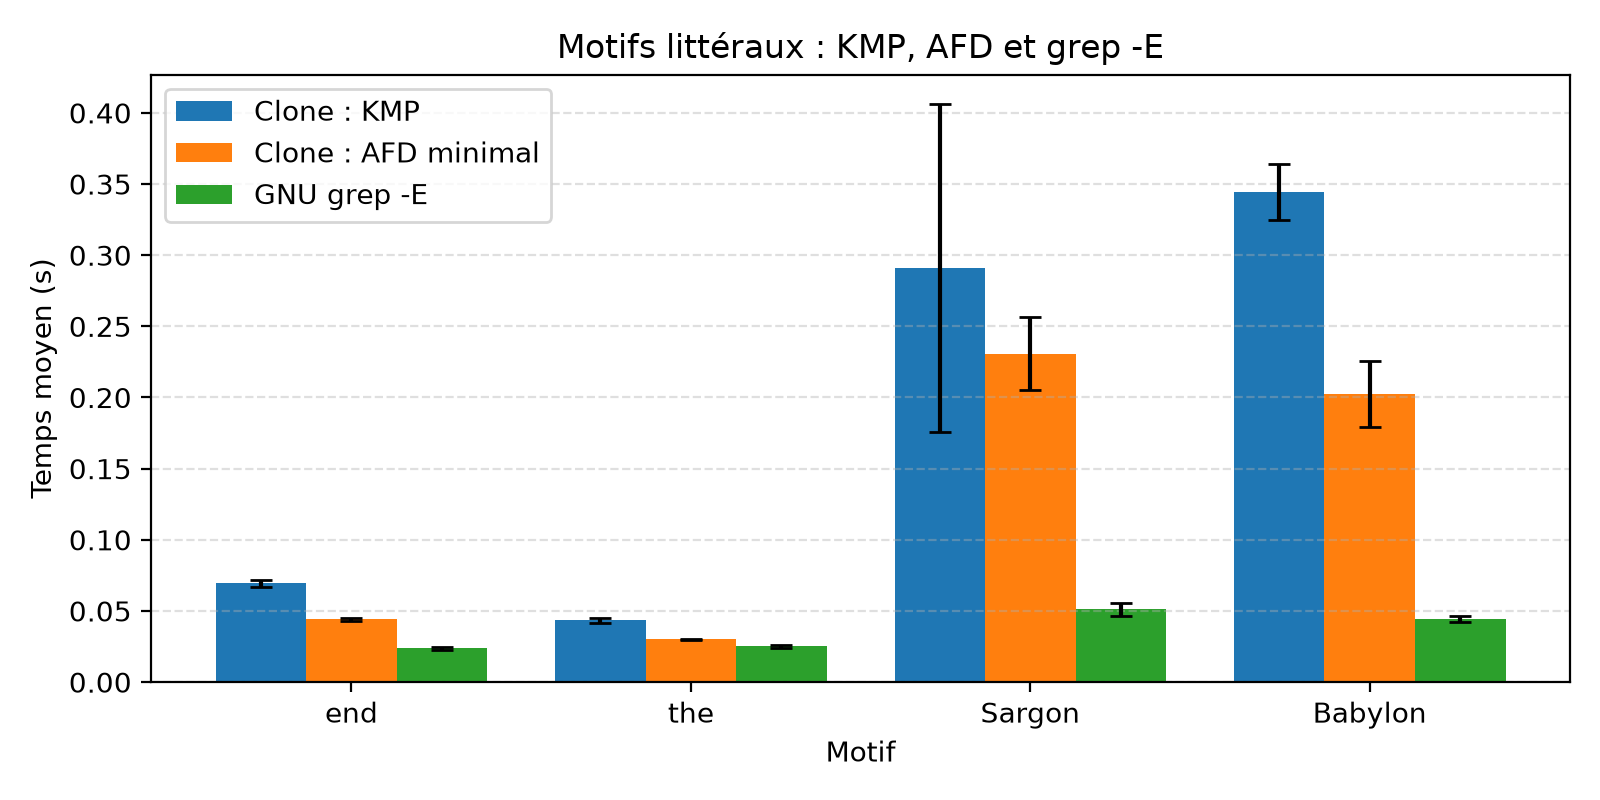
\includegraphics[width=0.85\textwidth]{benchmark_literal.png}
\caption{Motifs littéraux~: KMP, AFD minimal et \texttt{grep -E}
(moyenne et écart-type sur 10 exécutions).}
\label{fig:literal}
\end{figure}

\begin{figure}[ht]
\centering
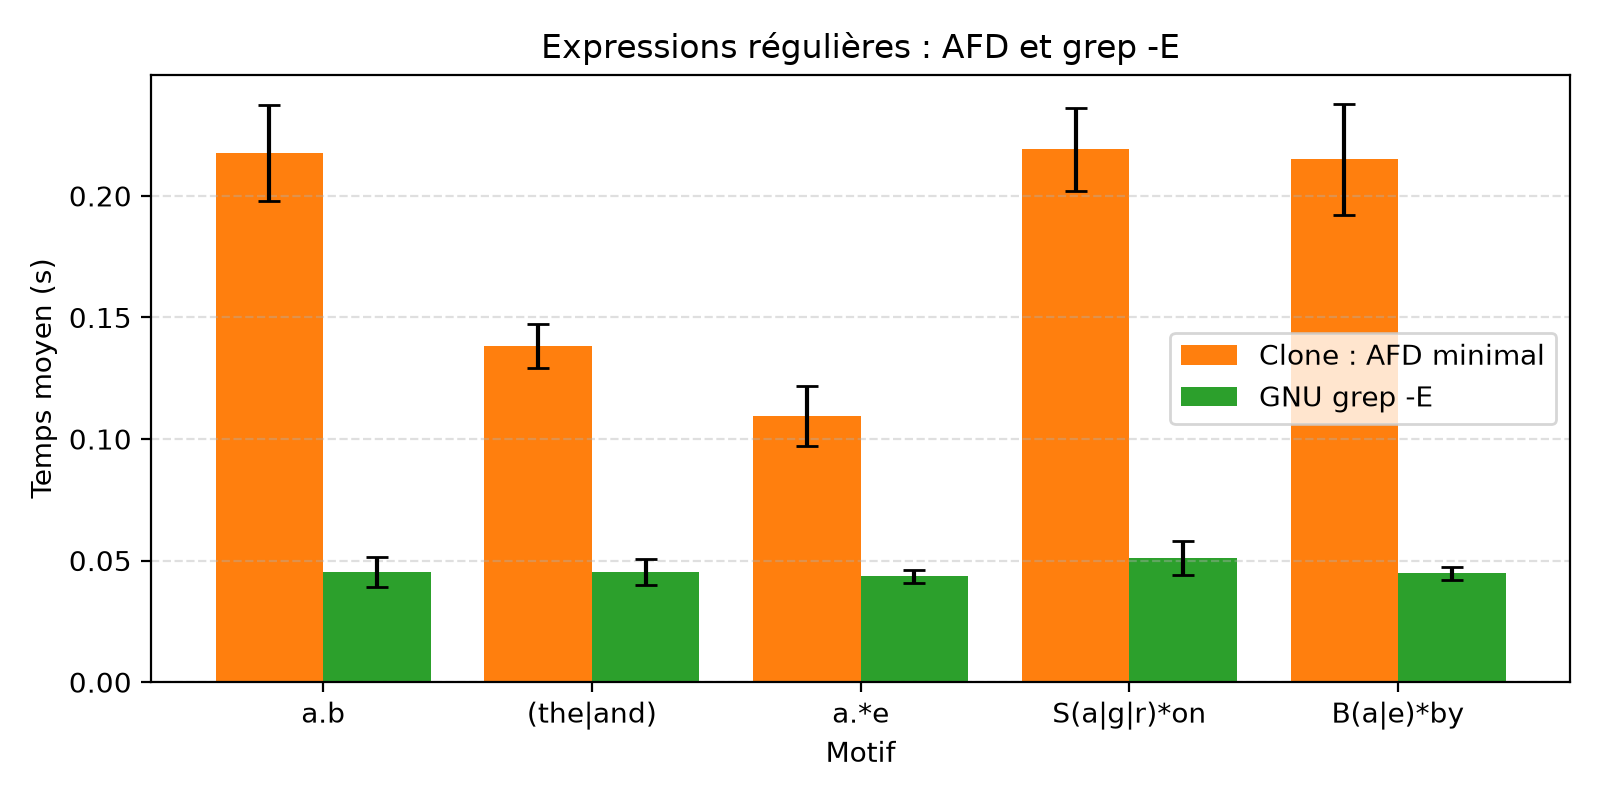
\includegraphics[width=0.85\textwidth]{benchmark_regex.png}
\caption{Expressions régulières~: AFD minimal et \texttt{grep -E}
(moyenne et écart-type sur 10 exécutions).}
\label{fig:regex}
\end{figure}

\paragraph{KMP contre automate (figure~\ref{fig:literal}).} Sur les quatre
motifs littéraux, l'AFD minimal est plus rapide que KMP dans notre
implémentation~: par exemple 0,20~s contre 0,34~s pour \texttt{Babylon} et
0,044~s contre 0,069~s pour \texttt{end}. Comme prévu en
section~\ref{sec:analyse}, les deux méthodes sont linéaires~; la différence
vient du coût par caractère en Python (une consultation de dictionnaire pour
l'AFD, plusieurs comparaisons et mises à jour d'indices pour KMP), le coût de
construction de l'AFD étant négligeable pour un motif court. Le routage vers
KMP n'apporte donc pas de gain de temps ici~; son avantage est d'éviter la
déterminisation et de garantir un prétraitement en $O(m)$.

\paragraph{Clone contre \texttt{grep} (figures~\ref{fig:literal} et~\ref{fig:regex}).}
\texttt{grep -E} est plus rapide pour tous les motifs~: environ 0,02 à 0,05~s,
dont environ 0,022~s de lancement du processus (mesuré sur un fichier vide),
contre 0,03 à 0,23~s pour l'AFD (jusqu'à 5 fois plus lent). L'écart est le plus faible pour
les motifs fréquents (\texttt{the}, \texttt{a.*e}), car l'arrêt à la première
occurrence évite de lire la fin de la plupart des lignes~; il est maximal pour
les motifs rares (\texttt{a.b}, \texttt{S(a|g|r)*on}), pour lesquels chaque
ligne est lue entièrement. \texttt{grep} est écrit en C, travaille sur des
blocs d'octets plutôt que ligne par ligne et utilise un AFD paresseux ainsi
que Boyer-Moore pour sauter des portions du texte. Le temps du clone dépend
peu du motif à fréquence égale, ce qui est cohérent avec une recherche en
$O(n)$ indépendante de la taille de l'automate.

% ------------------------------------------------------------------------------
\section{Conclusion et perspectives}
% ------------------------------------------------------------------------------

Nous avons réalisé un clone de \texttt{egrep} pour le sous-ensemble demandé
des ERE, qui implémente la chaîne complète de la Séance~1 (arbre syntaxique,
AFN d'Aho-Ullman, AFD par sous-ensembles, minimisation, recherche) et
l'algorithme KMP de la Séance~2 pour les motifs littéraux. Ses sorties sont
identiques à celles de \texttt{grep -E} sur les 22 cas testés. Les mesures
montrent un temps de recherche linéaire, un AFD minimal plus rapide que KMP en
Python, et un écart de performance avec \texttt{grep} dû principalement au
langage et aux optimisations de bas niveau de \texttt{grep}.

Plusieurs pistes permettraient d'aller plus loin~: compléter la norme ERE
(\texttt{+}, \texttt{?}, classes de caractères, ancres, échappements)~;
construire l'AFD paresseusement pour éviter l'explosion exponentielle~;
utiliser un algorithme de type Boyer-Moore pour les littéraux et pour filtrer
les lignes à l'aide d'un facteur obligatoire du motif. Enfin, dans le cas
\emph{offline} d'un fichier fixe interrogé de nombreuses fois, un précalcul
d'une table d'index des mots du texte (\emph{forward indexing}), stockée dans
un fichier cache et interrogée via un trie, une table de hachage ou un filtre
de Bloom, permettrait de ne parcourir que les lignes susceptibles de
contenir le motif.

\bibliographystyle{plainnat}
\bibliography{references}

\end{document}
